\begin{figure}[t]
\centering
\tikzstyle{every node}=[text centered, font=\small, inner sep=1pt]
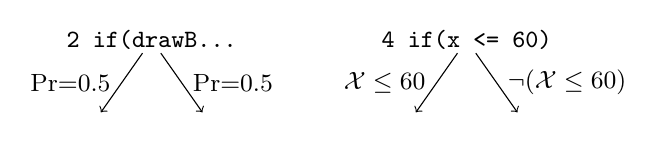
\begin{tikzpicture}[scale=0.38, level/.style={sibling distance = 25mm, level distance = 20mm}]
  \node[xshift=0mm] {\texttt{2 if(drawB...}}
    child{
      node[yshift=-2mm, xshift=-2mm] {}
      edge from parent[->]
      node[left,xshift=-1mm] {\small Pr=0.5}
    }
    child{
      node[yshift=-2mm, xshift=2mm] {}
      edge from parent[->]
      node[right,xshift=1mm] {\small Pr=0.5}
  };

  \node[xshift=40mm] {\texttt{4 if(x <= 60)}}
    child{
      node[yshift=-2mm, xshift=-2mm] {}
      edge from parent[->]
      node[left,xshift=-1mm] {\small ${\cal X} \le 60$}
    }
    child{
      node[yshift=-2mm, xshift=2mm] {}
      edge from parent[->]
      node[right,xshift=1mm] {\small $\neg({\cal X} \le 60)$}
  };
\end{tikzpicture}
\caption{Probabilistic Choice (left) and Symbolic Choice (right)}
\label{fig:choice}
\end{figure}

